\section{System Requirements Specification}

\subsection{Purpose}
This is the software requirement specification for the new version of Stedr, both the backend system that provides content and also the frontend that shows the content and the context of the content to the user. Here the traditional architectural terms backend - and frontend are used, but there are some subtleties to this term, as the frontend itself is managing a content service of its own. 

\subsection{Intended audience and reading suggestions}
Intended readers for this document are current and future developers, and the customer. The reader should also be noted that the SRS both can be read as a stand-alone document to get an overview of the rationalization behind the development process, but that it also is a part of the project report as a whole


\subsection{References}
The software requirements are based on the standard as provided by ISO/IEC:25010 \cite[10]{25010}, and also the models that can be found in this report’s section for architecture and modelling. References to the ISO-standard and other literature are found at the end of the project report under references.

\subsection{Product perspective}
Originally Stedr is a product developed by students at NTNU as a part of the subject TDT4290, and this application will form a basis for out continued development. The state of the exisiting application is considered to be a working prototype, and to some degrees it is an application that is built up with a traditonal server-client architecture. A simple technical overview of the system is provided below. 

\begin{figure}[h!]
\begin{center}
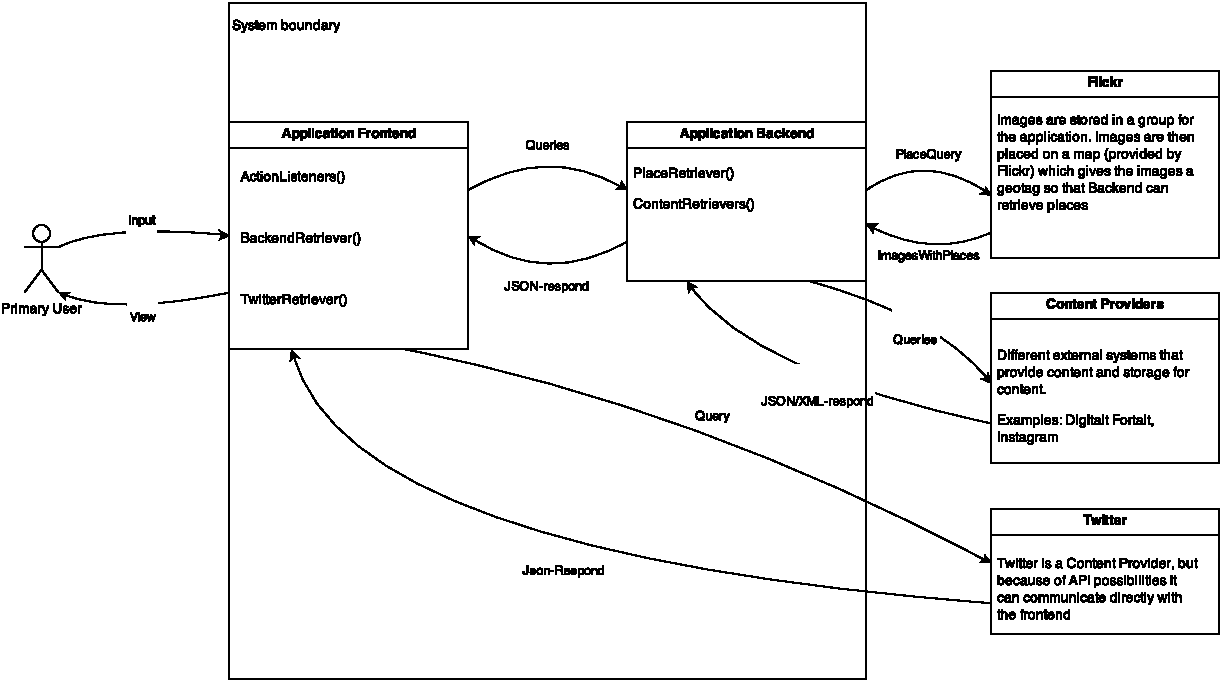
\includegraphics[scale=0.6]{tooverview-architecture}
\caption{A simple technical overview of the architecture}
\end{center}
\end{figure}

\subsection{User classes and charateristics}
The users of the program mainly divide into two categories. One is the primary user group which are using the frontend to see content. A typical user of this sort is a highschool student which is introduced to the program in the context of cultural heritage awareness. Most of these student will likely not use the program outside of the school context, but there is a possiblity that some of these students transits to the second category. Under the second category there are two user types, one is the content providers and the other is the maintainer. 
(See another section)

\subsection{Operating environment}
The frontend application of the system is a mobile application which aims to run on both the Android and iOS platform. Because of difficulties with developing towards the iOS platform without equipment from Apple, it's still discussed how the system is going to be tested on iOS. The backend of the server running as a server application, provided by Heroku.


\subsection{Product functions}

\subsection{Design and Implementation Constraints}

\subsection{User Documentation}

\subsection{Assumptions and Dependencies}
 
\subsection{External Interface Requirements}

\subsection{User Interfaces}
 
\subsection{Hardware Interfaces}
 
\subsection{Software Interfaces}

\subsection{System Features}

\clearpage

\begin{center}
\begin{tabular}{i{4cm}|| i{10cm}} \toprule

\multicolumn{2}{c}{\textbf{SF-1}} \\ \hline

Name & Find place on map \\ \hline
Priority & H \\ \hline
Goal & To browse the map to find a given place \\ \hline
Actors & Primary User \\ \hline
Preconditions & \begin{enumerate}  \item The home screen is displayes  \item The internal system and external systems are running \item The device has a internet connection  \end{enumerate} \\ \hline
Stimulus-Response  &  \begin{enumerate}  \item The home screen is displayes  \item The internal system and external systems are running \item The device has a internet connection  \end{enumerate} \\ \hline
Alternate Flow & \begin{itemize} \item[2a] The place does not exist and is not shown on the map \end{itemize} \\ \hline
Functional Requirement & A user should be able to access and browse a map, with places as pinpoints at their respective geographical location. The pinpoints should contain the picture and information found on Flickr. Group places close to eachother in one icon on map. \\ \hline
Related Use Cases & 1,3 \\ \hline
Dependencies & none \\ \bottomrule

\end{tabular}
\end{center}

\begin{center}
\begin{tabular}{i{4cm}|| i{10cm}} \toprule

\multicolumn{2}{c}{\textbf{SF-2}} \\ \hline

Name & Open menu \\ \hline
Priority & H \\ \hline
Goal & Open the drawer menu  \\ \hline
Actors & Primary User \\ \hline
Preconditions & \begin{enumerate} \item 2,3 \item[4] A screen with the menu button \end{enumerate} \\ \hline
Stimulus-Response & \begin{enumerate} \item The user clicks the menu button \item The menu opens \end{enumerate} \\ \hline
Alternate Flow & \begin{itemize} \item[1a] The user clicks the menu button, and the menu is already open \item[2a] The menu closes \end{itemize} \\ \hline
Functional Requirement & A button with the possibility to open the menu should always be presented to the user, so that the user easily can navigate the application. \\ \hline
Related Use Cases & 1,2 \\ \hline
Dependencies & none \\ \bottomrule

\end{tabular}
\end{center}

\begin{center}
\begin{tabular}{i{4cm}|| i{10cm}} \toprule

\multicolumn{2}{c}{\textbf{SF-3}} \\ \hline

Name & Search for a location \\ \hline
Priority & M \\ \hline
Goal & Go to a location on the map \\ \hline
Actors & Primary User \\ \hline
Preconditions & \begin{enumerate} \item 1,2,3 \end{enumerate} \\ \hline
Stimulus-Response & \begin{enumerate} \item The user searches for a location with the search bar in the map view. \item The map navigates to the location \end{enumerate} \\ \hline
Alternate Flow & \begin{itemize} \item[2a] Location is not found and is not navigated to. \end{itemize} \\ \hline
Functional Requirement & A search bar related to the map should be presented to the user, so the user can search for locations (independent of places) to see if there are any stories at that place. \\ \hline
Related Use Cases & 1 \\ \hline
Dependencies & none \\ \bottomrule

\end{tabular}
\end{center}

\begin{center}
\begin{tabular}{i{4cm}|| i{10cm}} \toprule

\multicolumn{2}{c}{\textbf{SF-4}} \\ \hline

Name & Refresh map \\ \hline
Priority & H \\ \hline
Goal & Update the map with content. \\ \hline
Actors & Primary User \\ \hline
Preconditions & \begin{enumerate} \item 1,2,3 \end{enumerate} \\ \hline
Stimulus-Response & \begin{enumerate} \item The user clicks the update button. \item The map refreshes and show new places \end{enumerate} \\ \hline
Alternate Flow & \begin{itemize} \item[2a] No new places are found, so no places are added to the map. \end{itemize} \\ \hline
Functional Requirement & The user should be presented with a button that makes requests for new places with content when pushed. This function should also be done automatically so that new content is sent to the user within 5 minutes after it’s added. \\ \hline
Related Use Cases & 1 \\ \hline
Dependencies & none \\ \bottomrule

\end{tabular}
\end{center}

\begin{center}
\begin{tabular}{i{4cm} ||  i{10cm}} \toprule

\multicolumn{2}{c}{\textbf{SF-5}} \\ \hline

Name & Go to location \\ \hline
Priority & H \\ \hline
Goal & Go to users location. \\ \hline
Actors & Primary User \\ \hline
Preconditions & \begin{enumerate} \item 1,2,3 \end{enumerate} \\ \hline
Stimulus-Response & \begin{enumerate} \item The user clicks the gps button. \item The map zooms to the users location.  \end{enumerate} \\ \hline
Alternate Flow & \begin{itemize} \item[2a] GPS not available so it can’t go to the users location. \end{itemize} \\ \hline
Functional Requirement & Since the user has the possibility to navigate the map freely, it should also be possible to quickly navigate to places relevant (in context of location) to him/her. \\ \hline
Related Use Cases & 1 \\ \hline
Dependencies & none \\ \bottomrule

\end{tabular}
\end{center}

\begin{center}
\begin{tabular}{i{4cm}|| i{10cm}} \toprule

\multicolumn{2}{c}{\textbf{SF-6}} \\ \hline

Name & Open views \\ \hline
Priority & H \\ \hline
Goal & Open views and see the content related to that specific view \\ \hline
Actors & Primary User \\ \hline
Preconditions & \begin{enumerate} \item 1,2,3 \end{enumerate} \\ \hline
Stimulus-Response & \begin{enumerate} \item The user clicks on a view \item The user changes views at will \item Content  \end{enumerate} \\ \hline
Alternate Flow & \begin{itemize} \item[1a] If the user clicks a button for the already chosen view, nothing should happen. \end{itemize} \\ \hline
Functional Requirement & For navigation in the place view, the user should be presented with different buttons (or tabs) so that the user easily can navigate between content and still have an overview of what types of content the application provides. Preview picture gallery when places are grouped together. Add description about place, own vire for sound. Be able to show place location on map from story. Be able to filter stories by tag, author, institution video/no video. preview stories by sound from SoundCloud \\ \hline
Related Use Cases & 3 \\ \hline
Dependencies & none \\ \bottomrule

\end{tabular}
\end{center}

\begin{center}
\begin{tabular}{i{4cm}|| i{10cm}} \toprule

\multicolumn{2}{c}{\textbf{SF-7}} \\ \hline

Name & Load content \\ \hline
Priority & H \\ \hline
Goal & Content is loaded from the external systems \\ \hline
Actors & Internal System \\ \hline
Preconditions & \begin{enumerate} \item 1,2,3 \end{enumerate} \\ \hline
Stimulus-Response & \begin{enumerate} \item Access the server as done in the previous version of the system \item Provide input to the server “placeId=” \item Content is loaded and a JSON-object is replied by the server \end{enumerate} \\ \hline
Alternate Flow & \begin{itemize} \item[1a] If the user clicks a button for the already chosen view, nothing should happen. \end{itemize} \\ \hline
Functional Requirement & The API for DF has to be changed, without changing the behaviour of the response from the server. In additon to this the server will respond with a new container for the audio content. Other content should be handled as normal. Retrieve collectionfrom DF based on hashtag and location.  Retrieve stories in a collection from DF based on tags. Open info retrived from SoundCloud based on hashtags or location. Retrieve information from Instagram based on Hashtags. Be able to get tinyUrls to different content. \\ \hline
Related Use Cases & Null \\ \hline
Dependencies & none \\ \bottomrule

\end{tabular}
\end{center}

\begin{center}
\begin{tabular}{i{4cm}|| i{10cm}} \toprule

\multicolumn{2}{c}{\textbf{SF-8}} \\ \hline

Name & Collection \\ \hline
Priority & H \\ \hline
Goal & Get all places related to a theme. \\ \hline
Actors & Primary User \\ \hline
Preconditions & \begin{enumerate} \item 1,2,3 \end{enumerate} \\ \hline
Stimulus-Response & \begin{enumerate} \item Access the menu bar. \item Click on the Collections-button \item Choose a collection \item Collections view is opened \item Change to map view \item Places related to the collections is shown on map \end{enumerate} \\ \hline
Alternate Flow & \begin{itemize} \item[3a] No Collections are available \end{itemize} \\ \hline
Functional Requirement & A container called Collections are to be implemented. Collections. Allow switching between map-related and collection related funtionallity. Display picture, title and description about a collection. Have a storyListView. Preview stories in collection story list. Open story in collection list. Places on map view with icon for each story in colelction. Preview a place for story on map.\\ \hline
Related Use Cases & 3 \\ \hline
Dependencies & none \\ \bottomrule

\end{tabular}
\end{center}

\begin{center}
\begin{tabular}{i{4cm}|| i{10cm}} \toprule

\multicolumn{2}{c}{\textbf{SF-9}} \\ \hline

Name & Upload content \\ \hline
Priority & M \\ \hline
Goal & Upload content \\ \hline
Actors & Primary User \\ \hline
Preconditions & \begin{enumerate} \item 1,2,3 \item[5] The user has an account at the content provider he or she is trying to upload to.  \item[6] Places related to the collections is shown on map \end{enumerate} \\ \hline
Stimulus-Response & \begin{enumerate} \item Access the tabs for different views \item Click the add-button in the views. \end{enumerate} \\ \hline
Alternate Flow & \begin{itemize} \item[3a] No Collections are available \end{itemize} \\ \hline
Functional Requirement & The user should have the possibility to add content so that. Add picture directly from stedr. ask the user for login-credentials the first time, then store locally for continued access. A similar approach for SoundCloud. Have relevant hashtags copied to clipboard. Be able to comment and like pictures on instagram. \\ \hline
Related Use Cases & Null \\ \hline
Dependencies & none \\ \bottomrule

\end{tabular}
\end{center}

\begin{center}
\begin{tabular}{i{4cm}|| i{10cm}} \toprule

\multicolumn{2}{c}{\textbf{SF-10}} \\ \hline

Name & Get help and info \\ \hline
Priority & H \\ \hline
Goal & Be informed \\ \hline
Actors & Primary User \\ \hline
Preconditions & \begin{enumerate} \item 1,2,3  \end{enumerate} \\ \hline
Stimulus-Response & \begin{enumerate} \item Access the drawer menu \item Click the help button. \item Select the option for what help you need \end{enumerate} \\ \hline
Alternate Flow &  \\ \hline
Functional Requirement & Introduction for first users. Help available at any time.\\ \hline
Related Use Cases & Null \\ \hline
Dependencies & none \\ \bottomrule

\end{tabular}
\end{center}




\subsection{Product Quality}

Guided by ISO:25010, meetings with our supervisor and the feature list given to us by the customer the product qualities that are important for the project is functional suitability, portabilty and maintainability.

\subsubsection{Compatibility}


\subsubsection{Performance Efficiency}
Even though the system isn't a part of a critical operation, the new and improved system will have performance efficiency as an important model of quality. The reasoning behind this is that decreased response time between components in the system is specfically asked for at multiple places in the feature list provided by the customer. 

As of now the time to load new content from the content providers to the application is slow and random. Because of this there are no exact estimation on the time used to pull content from Digitalt Fortalt and Instagram, but the application should use no more than \textit{300 seconds} to pull new content. Unrelated to the goal of performance issue; the user should be informed that the application isn't a real-time application.

Requirements related to resources utilized by the application when performing it's tasks, are already met by the prototype. The new version of the application are bound also bound by these goals. Specifically the backend is bound by the resources provided by the 1x Heroku Cloud Platform. Because of the utilization of the Google Maps API, the resources frontend is limited to the bound given to the application from Google Maps. 

Regarding capacity used by the the application, there should be an improvement. Because the application is to be used on the go where there may not be any WiFi-hotspots, the application should restrain itself to dowload content that is unrelated to where the user is. Because of the varied content types, it is hard to set a defined limit in how much contents (in terms of megabytes) the application should download. The limitations given to the application will therefore be set by the equation: \\ 
\begin{center} 
$\textrm{Bound}=\textrm{Content from Digitalt Fortalt}+5\times\textrm{Content from Twitter}+10\times\textrm{Picture from Flickr}+5\times\textrm{Picture from Instagram}$
\end{center}

\subsubsection{Reliability}
Since the application is going to be online without a team responsible for the technical maintenance, the server should be operative as long as the external content providers are feeding it with content. 

Because of the early versioning of the application, the aspect of maturity is not important for this application. Users of the application are few, and they know what the capabilities of the application is. This means that a user follows a rigid pattern and within that pattern, the probability to execute faults is almost non-existing. Functionality outside that pattern is not supported and thereby it's impossible to execute mistakes.

An important charecteristic of the application is that it has to be available just as often as a professional service. This means that under normal circumstances, the uptime of the backend and front should be 99 \%

Whenever faults are occuring, it is crucial that the backend has implemented services so that it can recover without the need of a maintainer. Because of the relative simplicity of the backend, the server should restart itself within \textit{180 seconds}

\subsubsection{Portability}

It is important to the customer that the application is made available on multiple platform as this is a demand by Tag Cloud. The minimal number of platforms which the product should run on is iOS and Android. 

Following this, the frontend of the application should be written once and compiled down to both the iOS and Android platform. The backend should provide agnostic responses, so that the responses can be handled the same by on Android and iOS devices. 

Because of the early development phase of the application, there is not a requirement to install the application from the normal application providers Google Play and Apple Store. It is enough that it is possible to install the applications on development devices. This also leads to that the application doesn't need to consider replaceability at this point.  



